% Options for packages loaded elsewhere
\PassOptionsToPackage{unicode}{hyperref}
\PassOptionsToPackage{hyphens}{url}
\PassOptionsToPackage{dvipsnames,svgnames,x11names}{xcolor}
%
\documentclass[
  letterpaper,
  DIV=11,
  numbers=noendperiod]{scrartcl}

\usepackage{amsmath,amssymb}
\usepackage{iftex}
\ifPDFTeX
  \usepackage[T1]{fontenc}
  \usepackage[utf8]{inputenc}
  \usepackage{textcomp} % provide euro and other symbols
\else % if luatex or xetex
  \usepackage{unicode-math}
  \defaultfontfeatures{Scale=MatchLowercase}
  \defaultfontfeatures[\rmfamily]{Ligatures=TeX,Scale=1}
\fi
\usepackage{lmodern}
\ifPDFTeX\else  
    % xetex/luatex font selection
\fi
% Use upquote if available, for straight quotes in verbatim environments
\IfFileExists{upquote.sty}{\usepackage{upquote}}{}
\IfFileExists{microtype.sty}{% use microtype if available
  \usepackage[]{microtype}
  \UseMicrotypeSet[protrusion]{basicmath} % disable protrusion for tt fonts
}{}
\makeatletter
\@ifundefined{KOMAClassName}{% if non-KOMA class
  \IfFileExists{parskip.sty}{%
    \usepackage{parskip}
  }{% else
    \setlength{\parindent}{0pt}
    \setlength{\parskip}{6pt plus 2pt minus 1pt}}
}{% if KOMA class
  \KOMAoptions{parskip=half}}
\makeatother
\usepackage{xcolor}
\setlength{\emergencystretch}{3em} % prevent overfull lines
\setcounter{secnumdepth}{-\maxdimen} % remove section numbering
% Make \paragraph and \subparagraph free-standing
\makeatletter
\ifx\paragraph\undefined\else
  \let\oldparagraph\paragraph
  \renewcommand{\paragraph}{
    \@ifstar
      \xxxParagraphStar
      \xxxParagraphNoStar
  }
  \newcommand{\xxxParagraphStar}[1]{\oldparagraph*{#1}\mbox{}}
  \newcommand{\xxxParagraphNoStar}[1]{\oldparagraph{#1}\mbox{}}
\fi
\ifx\subparagraph\undefined\else
  \let\oldsubparagraph\subparagraph
  \renewcommand{\subparagraph}{
    \@ifstar
      \xxxSubParagraphStar
      \xxxSubParagraphNoStar
  }
  \newcommand{\xxxSubParagraphStar}[1]{\oldsubparagraph*{#1}\mbox{}}
  \newcommand{\xxxSubParagraphNoStar}[1]{\oldsubparagraph{#1}\mbox{}}
\fi
\makeatother


\providecommand{\tightlist}{%
  \setlength{\itemsep}{0pt}\setlength{\parskip}{0pt}}\usepackage{longtable,booktabs,array}
\usepackage{calc} % for calculating minipage widths
% Correct order of tables after \paragraph or \subparagraph
\usepackage{etoolbox}
\makeatletter
\patchcmd\longtable{\par}{\if@noskipsec\mbox{}\fi\par}{}{}
\makeatother
% Allow footnotes in longtable head/foot
\IfFileExists{footnotehyper.sty}{\usepackage{footnotehyper}}{\usepackage{footnote}}
\makesavenoteenv{longtable}
\usepackage{graphicx}
\makeatletter
\newsavebox\pandoc@box
\newcommand*\pandocbounded[1]{% scales image to fit in text height/width
  \sbox\pandoc@box{#1}%
  \Gscale@div\@tempa{\textheight}{\dimexpr\ht\pandoc@box+\dp\pandoc@box\relax}%
  \Gscale@div\@tempb{\linewidth}{\wd\pandoc@box}%
  \ifdim\@tempb\p@<\@tempa\p@\let\@tempa\@tempb\fi% select the smaller of both
  \ifdim\@tempa\p@<\p@\scalebox{\@tempa}{\usebox\pandoc@box}%
  \else\usebox{\pandoc@box}%
  \fi%
}
% Set default figure placement to htbp
\def\fps@figure{htbp}
\makeatother

<style>
p,ul {
  font-size: 0.60em;
}
</style>
\KOMAoption{captions}{tableheading}
\makeatletter
\@ifpackageloaded{caption}{}{\usepackage{caption}}
\AtBeginDocument{%
\ifdefined\contentsname
  \renewcommand*\contentsname{Table of contents}
\else
  \newcommand\contentsname{Table of contents}
\fi
\ifdefined\listfigurename
  \renewcommand*\listfigurename{List of Figures}
\else
  \newcommand\listfigurename{List of Figures}
\fi
\ifdefined\listtablename
  \renewcommand*\listtablename{List of Tables}
\else
  \newcommand\listtablename{List of Tables}
\fi
\ifdefined\figurename
  \renewcommand*\figurename{Figure}
\else
  \newcommand\figurename{Figure}
\fi
\ifdefined\tablename
  \renewcommand*\tablename{Table}
\else
  \newcommand\tablename{Table}
\fi
}
\@ifpackageloaded{float}{}{\usepackage{float}}
\floatstyle{ruled}
\@ifundefined{c@chapter}{\newfloat{codelisting}{h}{lop}}{\newfloat{codelisting}{h}{lop}[chapter]}
\floatname{codelisting}{Listing}
\newcommand*\listoflistings{\listof{codelisting}{List of Listings}}
\makeatother
\makeatletter
\makeatother
\makeatletter
\@ifpackageloaded{caption}{}{\usepackage{caption}}
\@ifpackageloaded{subcaption}{}{\usepackage{subcaption}}
\makeatother

\usepackage{bookmark}

\IfFileExists{xurl.sty}{\usepackage{xurl}}{} % add URL line breaks if available
\urlstyle{same} % disable monospaced font for URLs
\hypersetup{
  pdftitle={Movimiento Circular y Repaso Ev. 1},
  pdfauthor={Flavio Jara L.},
  colorlinks=true,
  linkcolor={blue},
  filecolor={Maroon},
  citecolor={Blue},
  urlcolor={Blue},
  pdfcreator={LaTeX via pandoc}}


\title{Movimiento Circular y Repaso Ev. 1}
\author{Flavio Jara L.}
\date{}

\begin{document}
\maketitle


\subsection{Movimiento Circular}\label{movimiento-circular}

\subsection{Ejercicio 3}\label{ejercicio-3}

Usted está a cargo de una flota de vehículos de encomiendas. Uno de
éstos recoge insumos para llevarlos a su empresa que representa el
origen del sistema de referencia. Para ello, comienza el recorrido en la
central \(A\) ubicada a 15{[}km{]} y a N40°O (norte cuarenta grados
oeste) de la empresa. Luego de recoger los insumos en la central \(A\),
inicia el trayecto para llegar a la central \(B\) ubicada a N60°E de la
central \(A\) demorando 25{[}min{]} en llegar y viajando con una rapidez
de 50{[}km/h{]}. A continuación, inicia el trayecto para llegar a la
central \(C\), para lo cual, recorre 17{[}km{]} con una rapidez de 30
{[}km/h{]} y una dirección al S75°E. Finalmente, conduce a la empresa
demorando 0,7{[}h{]}.

De acuerdo con lo anterior, y considerando un sistema de referencia
ubicado en la empresa, responda:

\begin{itemize}
\tightlist
\item
  \begin{enumerate}
  \def\labelenumi{\alph{enumi})}
  \tightlist
  \item
    Por medio de vectores, dibuje la trayectoria seguida por el furgón
    de encomiendas.
  \end{enumerate}
\item
  \begin{enumerate}
  \def\labelenumi{\alph{enumi})}
  \setcounter{enumi}{1}
  \tightlist
  \item
    Determine los vectores de posición \(\vec{r}_a\), \(\vec{r}_b\) y
    \(\vec{r}_c\).
  \end{enumerate}
\item
  \begin{enumerate}
  \def\labelenumi{\alph{enumi})}
  \setcounter{enumi}{2}
  \tightlist
  \item
    Determine la velocidad media en todo el trayecto.
  \end{enumerate}
\item
  \begin{enumerate}
  \def\labelenumi{\alph{enumi})}
  \setcounter{enumi}{3}
  \tightlist
  \item
    Determine la rapidez media en todo el trayecto.
  \end{enumerate}
\end{itemize}

\subsection{}\label{section}

Definamos primero los vectores dados en el problema. \(\vec{r}_a\) es el
vector que va desde la empresa hasta la central \(A\), se nos da la
magnitud, la cual pasaremos a metros y el ángulo (el cual mediremos
desde el eje x), por lo que podemos escribirlo como: \[
\vec{r}_a = 15000 \cos(130°) \hat{ı} + 15000 \sin(130°) \hat{ȷ} \hspace{0.2cm} [m]
\] \[
\vec{r}_a = -9641.81 \hat{ı} + 11490.66 \hat{ȷ} \hspace{0.2cm} [m]
\]

\subsection{}\label{section-1}

Lo siguiente que nos dan es el vector que va desde la central \(A\)
hasta la central \(B\), el cual se encuentra a N60°E de la central
\(A\). No nos dan la magnitud, pero si la rapidez y el tiempo que demora
en llegar. Por lo que podemos calcular la magnitud del vector como: \[
v = \frac{d}{t} \Rightarrow d = v t
\] Pasando los kilómetros a metros y el tiempo a horas: \[
d = 50 \frac{km}{h} \cdot 25 min \cdot \frac{1 h}{60 min} \cdot 1000 \frac{m}{km}
\] \[
d = 20833.33 \hspace{0.2cm} [m]
\]

\subsection{}\label{section-2}

Ahora podemos escribir el vector \(\vec{r}_{ ab }\) como: \[
\vec{r}_{ab} = 20833.33 \cos(30°) \hat{ı} + 20833.33 \sin(30°) \hat{ȷ} \hspace{0.2cm} [m]
\] \[
\vec{r}_{ab} = 18042.5 \hspace{0.2cm} \hat{ı} + 10416.67 \hspace{0.2cm} \hat{ȷ} \hspace{0.2cm} [m]
\]

Con esto podemos sacar el vector \(\vec{r}_b\) como: \[
\vec{r}_b = \vec{r}_a + \vec{r}_{ab}
\] \[
\vec{r}_b = (-9641.81 \hspace{0.2cm} \hat{ı} + 11490.66 \hspace{0.2cm} \hat{ȷ}) + (18042.5 \hspace{0.2cm} \hat{ı} + 10416.67 \hspace{0.2cm} \hat{ȷ}) \hspace{0.2cm} [m]
\] \[
\vec{r}_b = 8400.69 \hspace{0.2cm} \hat{ı} + 21907.33 \hspace{0.2cm} \hat{ȷ} \hspace{0.2cm} [m]
\]

\subsection{}\label{section-3}

Ahora pasamos al vector que va desde la central \(B\) hasta la central
\(C\). Nos dan la magnitud y la dirección, por lo que podemos escribir
el vector como: \[
\vec{r}_{bc} = 17000 \cos(-15°) \hat{ı} + 17000 \sin(-15°) \hat{ȷ} \hspace{0.2cm} [m]
\] \[
\vec{r}_{bc} = 16420.74 \hspace{0.2cm} \hat{ı} - 4399.92 \hspace{0.2cm} \hat{ȷ} \hspace{0.2cm} [m]
\] Con esto podemos sacar el vector \(\vec{r}_c\) como: \[
\vec{r}_c = \vec{r}_b + \vec{r}_{bc}
\] \[
\vec{r}_c = (8400.69 \hspace{0.2cm} \hat{ı} + 21907.33 \hspace{0.2cm} \hat{ȷ}) + (16420.74 \hspace{0.2cm} \hat{ı} - 4399.92 \hspace{0.2cm} \hat{ȷ}) \hspace{0.2cm} [m]
\] \[
\vec{r}_c = 24821.43 \hspace{0.2cm} \hat{ı} + 17507.41 \hspace{0.2cm} \hat{ȷ} \hspace{0.2cm} [m]
\]

Finalmente, el vector que vuelve a la empresa es el vector
\(\vec{r}_{c}\), pero con dirección opuesta, por lo que podemos
escribirlo como: \[
\vec{r}_{ce} = -\vec{r}_c
\] \[
\vec{r}_{ce} = -24821.43 \hspace{0.2cm} \hat{ı} - 17507.41 \hspace{0.2cm} \hat{ȷ} \hspace{0.2cm} [m]
\]

\subsection{a)}\label{a}

Nos piden la trayectoria seguida por el furgón de encomiendas, por lo
que necesitamos graficar solo los vectores \(\vec{r}_{ab}\),
\(\vec{r}_{bc}\) y \(\vec{r}_{ce}\).

\pandocbounded{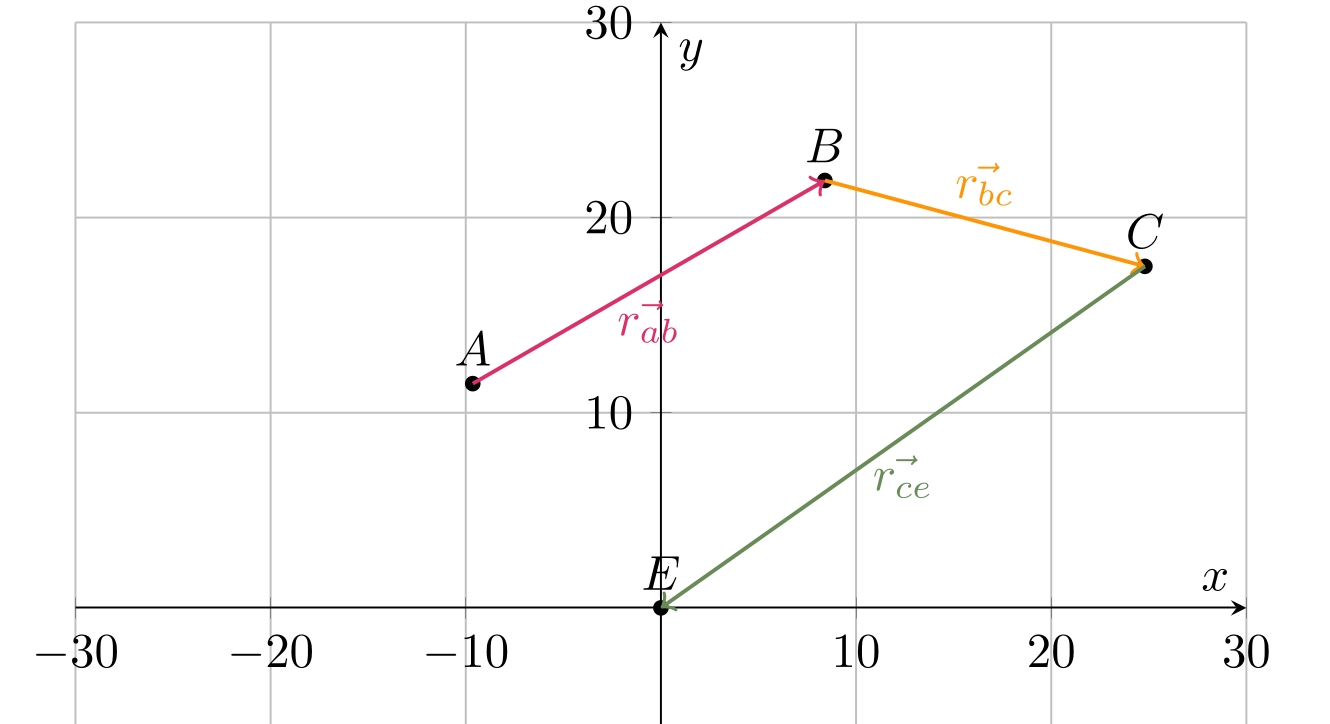
\includegraphics[keepaspectratio]{./1.png}}

\subsection{b)}\label{b}

Ya determinamos los vectores de posición \(\vec{r}_a\), \(\vec{r}_b\) y
\(\vec{r}_c\) en la parte anterior, por lo que no es necesario volver a
calcularlos.

\pandocbounded{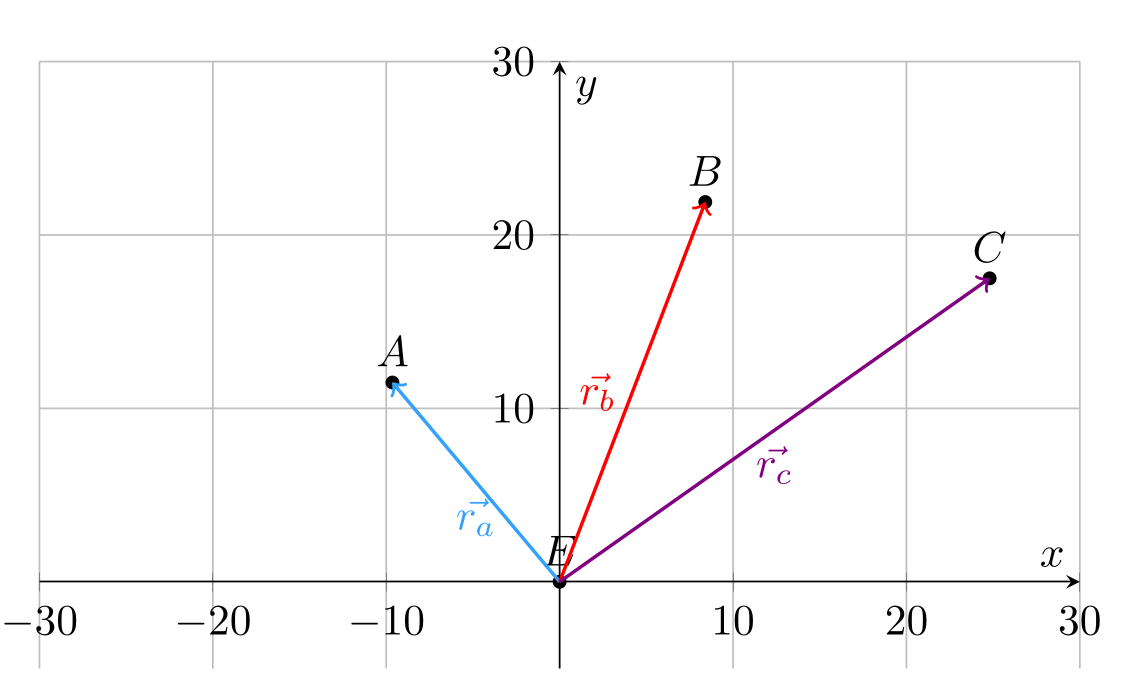
\includegraphics[keepaspectratio]{./2.png}}

\subsection{c)}\label{c}

Para determinar la velocidad media, debemos calcular el desplazamiento
total y el tiempo total. El desplazamiento total es la distancia entre
la posición inicial y la posición final, por lo que podemos escribirlo
como: \[
\vec{r}_{total} = \vec{r}_{ab} + \vec{r}_{bc} + \vec{r}_{ce}
\] \[
\vec{r}_{total} = (18042.5 \hspace{0.2cm} \hat{ı} + 10416.67 \hspace{0.2cm} \hat{ȷ}) + (16420.74 \hspace{0.2cm} \hat{ı} - 4399.92 \hspace{0.2cm} \hat{ȷ}) + (-24821.43 \hspace{0.2cm} \hat{ı} - 17507.41 \hspace{0.2cm} \hat{ȷ})
\] \[
\vec{r}_{total} = (18042.5 + 16420.74 - 24821.43) \hspace{0.2cm} \hat{ı} + (10416.67 - 4399.92 - 17507.41) \hspace{0.2cm} \hat{ȷ}
\] \[
\vec{r}_{total} = 9641.81 \hspace{0.2cm} \hat{ı} - 11490.66 \hspace{0.2cm} \hat{ȷ} \hspace{0.2cm} [m]
\] Sumamos todos los tiempos que demora el furgón en llegar a cada
central: \[
t_{total} = t_{ab} + t_{bc} + t_{ce}
\] No tenemos \(t_{bc}\), pero podemos calcularlo como:

\subsection{}\label{section-4}

\[
t_{bc} = \frac{d_{bc}}{v_{bc}} = \frac{17 \hspace{0.2cm} [km]}{30 \hspace{0.2cm} [km/h]} = 0.5667 \hspace{0.2cm} [h]
\] \[
t_{total} = 25 \hspace{0.2cm} [min] + 0.5667 \hspace{0.2cm} [h] + 0.7 \hspace{0.2cm} [h]
\] Pasando los minutos a horas: \[
t_{total} = 25 \hspace{0.2cm} [min] \cdot \frac{1 h}{60 min} + 0.5667 \hspace{0.2cm} [h] + 0.7 \hspace{0.2cm} [h]
\] \[
t_{total} = 0.4167 \hspace{0.2cm} [h] + 0.5667 \hspace{0.2cm} [h] + 0.7 \hspace{0.2cm} [h]
\] \[
t_{total} = 1.6834 \hspace{0.2cm} [h]
\] Pasandolo a segunods: \[
t_{total} = 1.6834 \hspace{0.2cm} [h] \cdot 3600 \hspace{0.2cm} [s/h] = 6060,24 \hspace{0.2cm} [s]
\]

\subsection{}\label{section-5}

Ahora podemos calcular la velocidad media como: \[
\vec{v}_{media} = \frac{\vec{r}_{total}}{t_{total}}
\]

\[
\vec{v}_{media} = \frac{9641.81 \hspace{0.2cm} \hat{ı} - 11490.66 \hspace{0.2cm} \hat{ȷ}}{6060,24 \hspace{0.2cm} [s]}
\] \[
\vec{v}_{media} = 1.59 \hspace{0.2cm} \hat{ı} - 1.9 \hspace{0.2cm} \hat{ȷ} \hspace{0.2cm} [m/s]
\]

\subsection{d)}\label{d}

La rapidez media el módulo de la velocidad media, por lo que podemos
escribirla como: \[
v_{media} = \sqrt{(1.59)^2 + (-1.9)^2}
\] \[
v_{media} = \sqrt{2.5281 + 3.61}
\] \[
v_{media} = \sqrt{6.1381} = 2.48 \hspace{0.2cm} [m/s]
\]

\subsection{Ejercicio 4}\label{ejercicio-4}




\end{document}
